\section{\LaTeX}
O \LaTeX é um sistema para a editoração de documentos de alta qualidade tipográfica. Utiliza-se do \TeX, um programa que foi criado pelo matemático Donald Knuth que, ao revisar o segundo volume da sua série de livros {\slshape The Art of Computer Programming} verificou que a sua qualidade era muito baixa e já que a produção de um texto em formato digital era basicamente uma combinação de zeros e uns (com tinta e sem tinta), decidiu criar um sistema próprio.

Knuth inicialmente previu que a sua tarefa, que consistia em aprender quais eram as formas tradicionais de se exibir fórmulas matemáticas, a maneira correta de se imprimir letras em um papel, como criar suas próprias fontes e por fim integrar tudo isso em um programa de computador, levaria aproximadamente 6 meses. Donald levou quase 10 anos e o produto final de seu trabalho foi o sistema \TeX \ e o programa de criação de fontes \textit{Metafont}.

\LaTeX é basedo na filosofia de que autores devem se focar no conteúdo sem precisar se preocupar com a apresentação visual do que estão escrevendo. Desta forma, ao escrever um documento usando \LaTeX, o autor precisa apenas especificar a estrutura lógica de seu texto, na forma de conceitos básicos como capítulos, seções, tabelas, figuras, etc. A apresentação fica a cargo do sistema.

%LaTeX can be arbitrarily extended by using the underlying macro language to develop custom formats. Such macros are often collected into packages, which are available to address special formatting issues such as complicated mathematical content or graphics. Indeed, in the example below, the align environment is provided by the amsmath package.

\subsection{Funcionamento}

O funcionamento do \LaTeX é o seguinte: a partir de um arquivo de texto com extensão \tex\ contendo comandos e o texto que se quer exibir, o programa \textsf{latex} produz um arquivo independente de plataforma \dvi. Este arquivo então é convertido para diversos formatos dependendo de sua utilização desejada. No caso de uso mais comum, o arquivo \dvi\ é convertido para \pdf. Para se evitar este processo de conversão, normalmente utiliza-se o comando \textsf{pdflatex} que gera o \pdf\ diretamente a partir do \tex.

Um exemplo de sintaxe dos comandos \TeX\ é visto a seguir:
\lstinputlisting{contents/exemplo.tex}

Este trecho de código produz um \pdf\ com esta aparência:

\noindent\makebox[\textwidth]{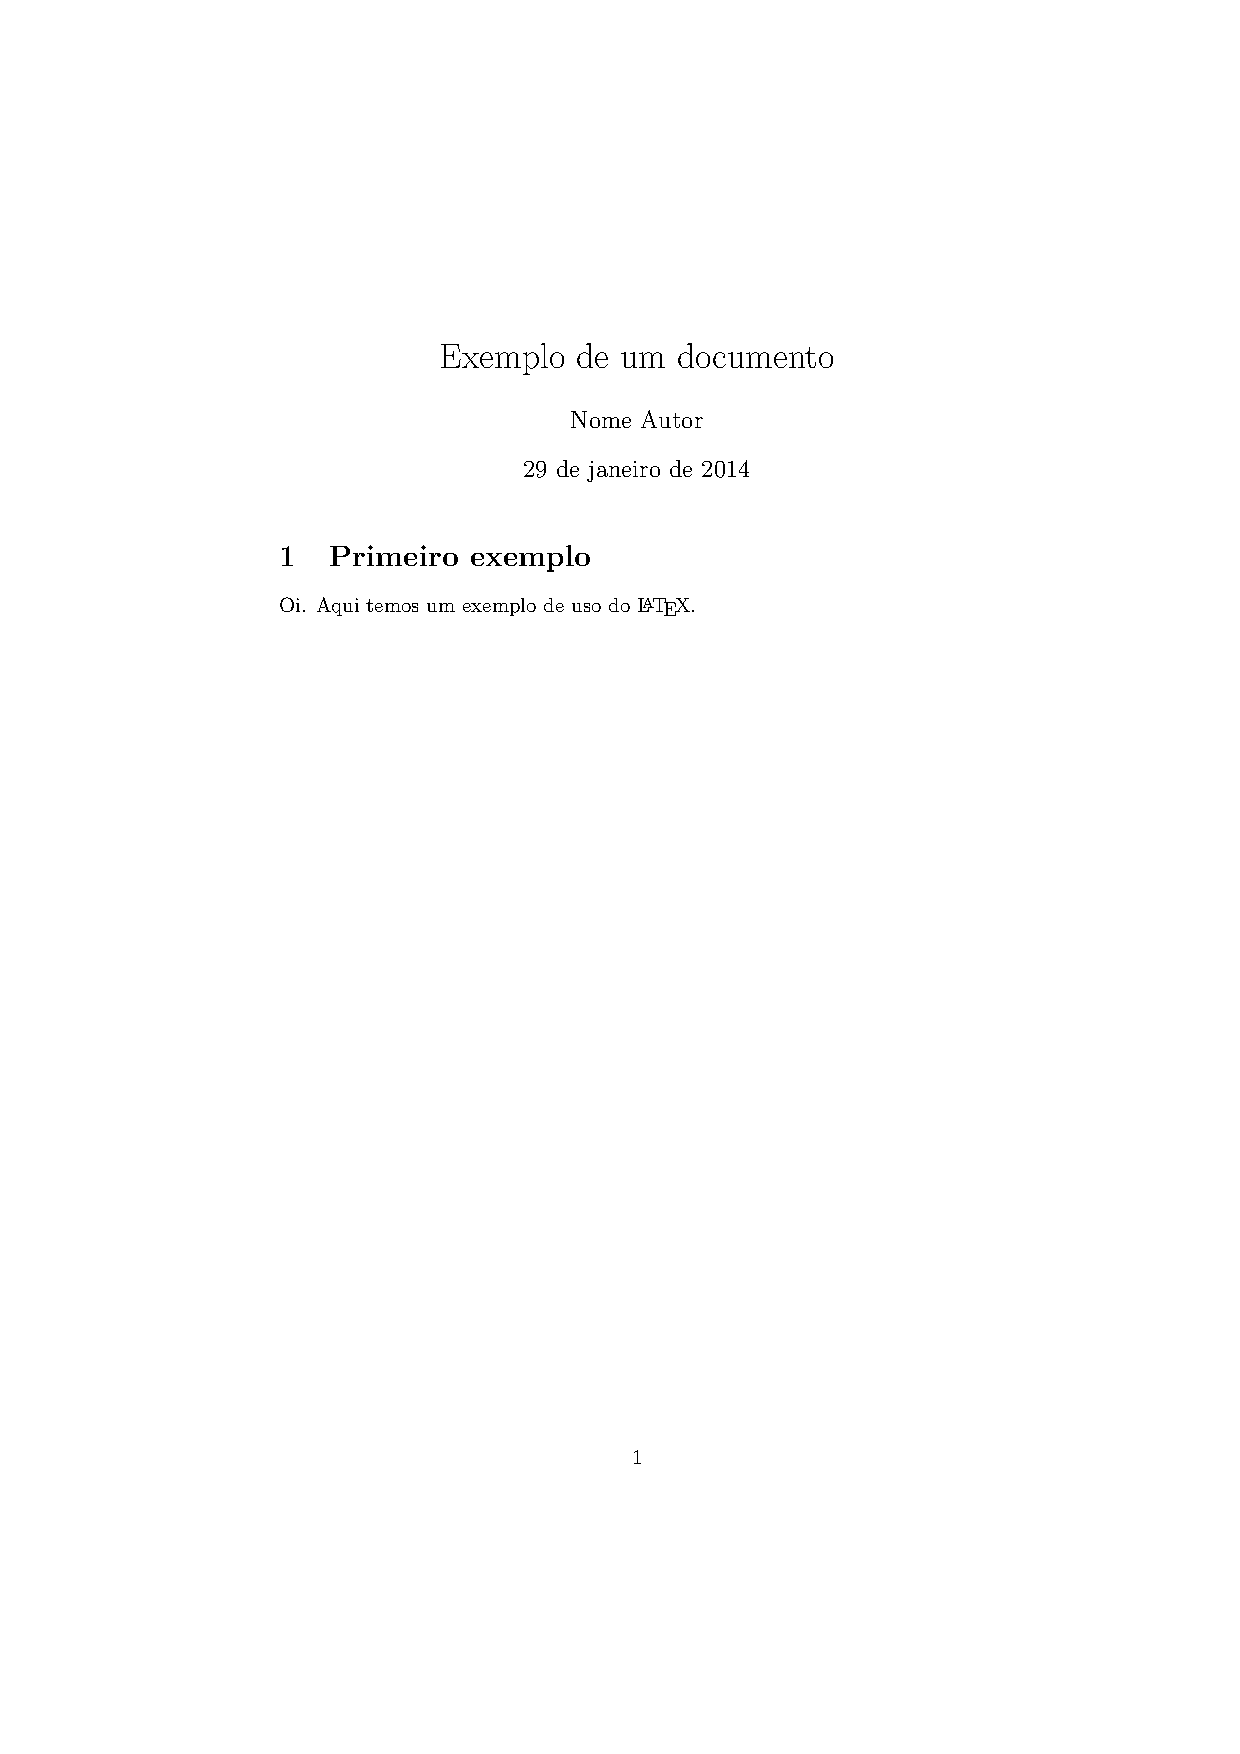
\includegraphics[trim= 0 18cm 0 5cm,clip]{contents/exemplo}}

Observe como, no código apresentado, não há nenhuma informação sobre que tipo de fonte utilizar, tamanho da letra, espaçamento entre linhas, posicionamento do título, etc. Estes detalhes são tratados pelo \LaTeX\ e o usuário não precisa se preocupar com eles.